\documentclass[11pt]{article}

\usepackage{amsmath,amssymb,mathtools}
\usepackage[margin=1in]{geometry}
\usepackage{enumitem}
\usepackage{xcolor}
\usepackage{microtype}
\usepackage{graphicx}
\usepackage{tikz,float}
\usepackage{subcaption}
\usepackage{amsthm}
\usepackage{hyperref}
\usepackage{array}
\usepackage{pgfplots}

\usetikzlibrary{shapes.geometric, arrows.meta, positioning, calc, decorations.markings}
\tikzset{
	block/.style={rectangle, draw, text width=6em, text centered, rounded corners, minimum height=10mm},
	sum/.style={circle, draw, node distance=1.5cm},
	line/.style={draw, -{Stealth[length=2.5mm, width=1.5mm]}}
}

\usepgfplotslibrary{groupplots}
\pgfplotsset{compat=1.18}

\pgfplotsset{
	myaxes/.style={
		axis lines=middle,
		axis line style={-latex},
		grid=major,
		grid style={gray!15},
		minor grid style={gray!35},
		xlabel style={at={(ticklabel* cs:1)}, anchor=north west},
		ylabel style={at={(ticklabel* cs:1)}, anchor=south east},
		every axis plot/.append style={thick}
	},
	myplotstyle/.style={
		width=14cm,
		height=7cm,
		axis lines=middle,
		axis line style={-Stealth},
		grid=both,
		minor tick num=1,
		major grid style={draw=gray!30},
		minor grid style={draw=gray!15},
		tick label style={font=\small, fill=white, inner sep=1.5pt},
		xlabel={$t$},
		ylabel={$x(t)$},
		xlabel style={anchor=north east, font=\small},
		ylabel style={anchor=south east, font=\small},
		samples=401,
	}
}

\newtheoremstyle{mynote}
{6pt}      % Space above
{6pt}      % Space below
{}          % Body font (normal, not italic)
{}          % Indent amount
{\bfseries} % Theorem head font
{.}         % Punctuation after theorem head
{.5em}      % Space after theorem head
{}          % Theorem head spec
\theoremstyle{mynote}
\newtheorem{definition}{Definition}
\newtheorem{proposition}{Proposition}
\newtheorem{example}{Example}
\newtheorem{remark}{Remark}
\newtheorem{theorem}{Theorem}
\newtheorem{corollary}{Corollary}

\newcommand{\T}{\mathcal{T}}
\newcommand{\R}{\mathbb{R}}
\newcommand{\Z}{\mathbb{Z}}
\newcommand{\C}{\mathbb{C}}
\newcommand{\conv}{\ast}
\newcommand{\dt}{\,\dd t}
\newcommand{\dd}{\mathrm{d}}
\newcommand{\imp}{\delta}
\newcommand{\sinc}[1]{\frac{\sin(\pi #1)}{\pi #1}}


\DeclareMathOperator{\rect}{rect}
\DeclareMathOperator{\Ev}{Ev}
\DeclareMathOperator{\Od}{Od}
\DeclareMathOperator{\sgn}{sgn}
\DeclareMathOperator{\step}{u}
\DeclareMathOperator{\tri}{tri}

\begin{document}
	% Reset figure counter for this lecture
	\renewcommand{\thefigure}{17.\arabic{figure}}
	
	% --- TITLE BLOCK ---
	\thispagestyle{empty}
	\noindent
	\begin{tabular*}{\textwidth}{l @{\extracolsep{\fill}} r}
		\textbf{Signals and Systems} & \textbf{Lecture 17} \\
		\textit{Dr. Ghandi Manasra and Ahmed Rabei} & \textit{Fall 2025} \\
	\end{tabular*}
	\hrule
	\vspace{0.4cm}
	\begin{center}
		\Large\textbf{Lecture 17: Magnitude and Phase Representation of the Fourier Transform}
	\end{center}
	\vspace{0.4cm}
	
\section*{Reference}
	Oppenheim \& Willsky, \textit{Signals and Systems}, Chapter 6, Section 6.1

\section*{Review of Lecture 16}
	\begin{itemize}[noitemsep]
		\item Duality properties of Fourier transforms
		\item Fourier transform tables and pairs
		\item Convolution property applications
		\item Today: magnitude and phase significance
	\end{itemize}

\section*{17.1 Introduction}

Over the past several weeks, we have developed a complete set of tools for transforming signals from the time domain to the frequency domain. We have the Fourier Series for periodic signals and the Fourier Transform for aperiodic signals, in both continuous and discrete time.

Today, we begin our deeper dive into the relationship between the time and frequency domains. We know that the Fourier transform, $X(j\omega)$, is a complex-valued function. We will now explore the significance of its \textbf{magnitude} and \textbf{phase} and what each part tells us about the original signal.

\subsection*{17.1.1 The Magnitude and Phase of the Fourier Transform}

The Fourier transform $X(j\omega)$ is a complex function of frequency, $\omega$. Just like any complex number, it can be represented in two principal forms:

\begin{definition}
	\textbf{Rectangular Form:}
	\[
	X(j\omega) = \operatorname{Re}\{X(j\omega)\} + j\operatorname{Im}\{X(j\omega)\}
	\]
	This form is often mathematically convenient for derivations.
\end{definition}

\begin{definition}
	\textbf{Polar Form:}
	\[
	X(j\omega) = |X(j\omega)|e^{j\angle X(j\omega)}
	\]
	This form is far more useful for building intuition.
\end{definition}

\begin{itemize}[noitemsep]
	\item \textbf{$|X(j\omega)|$} is the \textbf{magnitude} of the Fourier transform. It tells us "how much" of the frequency component $\omega$ is present in the signal. It is a non-negative, real function.
	\item \textbf{$\angle X(j\omega)$} is the \textbf{phase} of the Fourier transform. It tells us "how the different frequency components align in time" to create the signal's shape. It represents the relative time shift of each sinusoidal component. It is a real-valued function.
\end{itemize}

\paragraph{Mathematical Relationships:}
\begin{align}
|X(j\omega)| &= \sqrt{\operatorname{Re}\{X(j\omega)\}^2 + \operatorname{Im}\{X(j\omega)\}^2} \\
\angle X(j\omega) &= \operatorname{atan2}(\operatorname{Im}\{X(j\omega)\}, \operatorname{Re}\{X(j\omega)\})
\end{align}

For real-valued time signals $x(t)$, we know that $X(j\omega)$ is conjugate symmetric. This means:
\begin{itemize}[noitemsep]
	\item The magnitude $|X(j\omega)|$ is an \textbf{even function}: $|X(-j\omega)| = |X(j\omega)|$
	\item The phase $\angle X(j\omega)$ is an \textbf{odd function}: $\angle X(-j\omega) = -\angle X(j\omega)$
\end{itemize}

\begin{figure}[H]
	\centering
	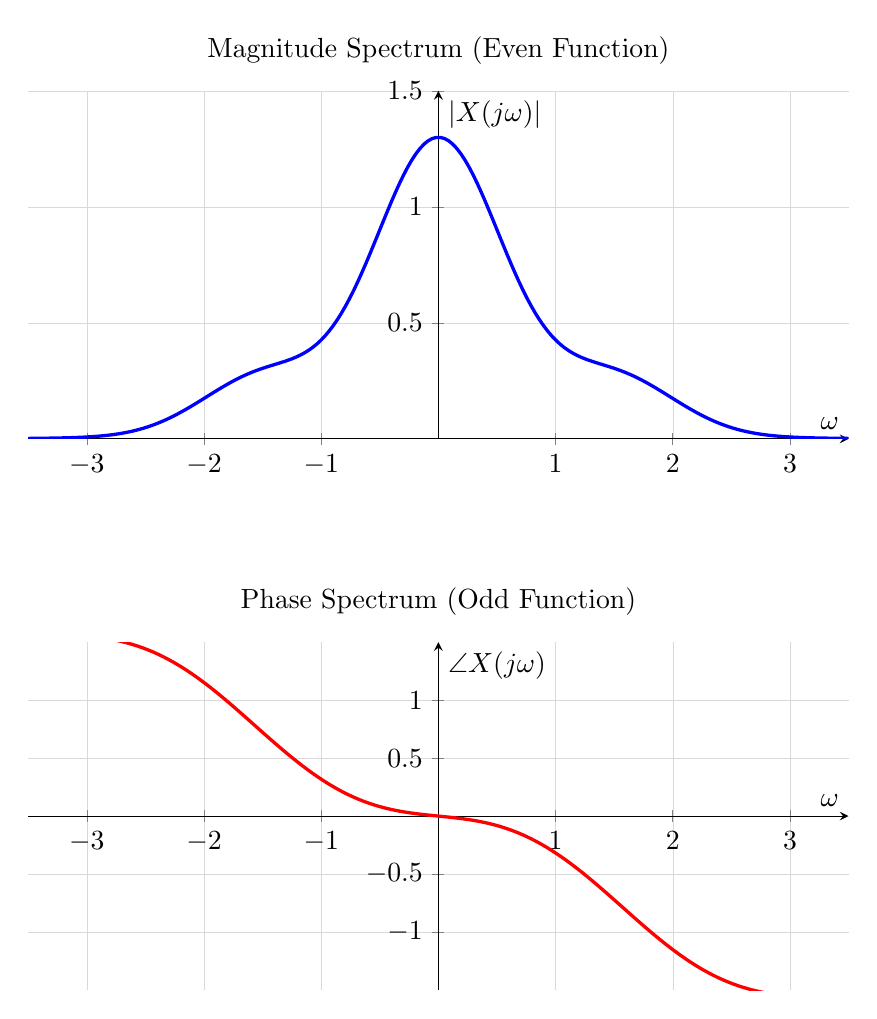
\begin{tikzpicture}
	% Define a common style for these plots
	\pgfplotsset{
		spec a/.style={
			width=12cm, height=6cm,
			axis lines=middle, xlabel={$\omega$},
			xmin=-3.5, xmax=3.5,
			xtick={-3, -2, -1, 1, 2, 3},
			grid=major, grid style={line width=.1pt, draw=gray!30},
			no marks,
		}
	}
	
	% Top plot: Magnitude
	\begin{scope}[yshift=7cm]
		\begin{axis}[
			spec a,
			title={Magnitude Spectrum (Even Function)},
			ylabel={$|X(j\omega)|$},
			ymin=0, ymax=1.5,
			ytick={0.5, 1, 1.5},
			]
			\addplot[blue, very thick, domain=-3.5:3.5, samples=200] {exp(-0.5*x^2) * (1 + 0.3*cos(deg(3*x)))};
		\end{axis}
	\end{scope}
	
	% Bottom plot: Phase
	\begin{scope}[yshift=0cm]
		\begin{axis}[
			spec a,
			title={Phase Spectrum (Odd Function)},
			ylabel={$\angle X(j\omega)$},
			ymin=-1.5, ymax=1.5,
			ytick={-1, -0.5, 0.5, 1},
			]
			\addplot[red, very thick, domain=-3.5:3.5, samples=200] {-0.5*x + 0.2*sin(deg(2*x))};
		\end{axis}
	\end{scope}
\end{tikzpicture}









	\caption{Magnitude and phase representation of a complex Fourier transform.}
	\label{fig:magnitude_phase_representation}
\end{figure}
\newpage
\section*{17.2 The Role of Magnitude and Phase}

The relative importance of magnitude and phase depends heavily on the application and the type of signal.

Consider a signal $x(t)$ and its Fourier transform $X(j\omega) = |X(j\omega)|e^{j\angle X(j\omega)}$.

Let's see what happens if we change the magnitude but keep the phase, and vice-versa:

\begin{itemize}[noitemsep]
	\item \textbf{Altering the Magnitude:} If we modify the magnitude to create a new spectrum $Y(j\omega) = |Y(j\omega)|e^{j\angle X(j\omega)}$, the resulting time signal $y(t)$ will have its frequency content changed, but the alignment and general location of features will be preserved.
	\item \textbf{Altering the Phase:} If we modify the phase to create a new spectrum $Z(j\omega) = |X(j\omega)|e^{j\angle Z(j\omega)}$, the resulting time signal $z(t)$ will have the same frequency content (the same power at each frequency), but the temporal structure can be completely destroyed.
\end{itemize}

\begin{remark}
	For many types of signals, particularly images and other signals where the temporal or spatial structure is critical, \textbf{the phase information is often more important than the magnitude information.} This principle was famously demonstrated by Oppenheim and Lim (1981) in their classic experiment where swapping the magnitude and phase spectra of two different images showed that the reconstructed image follows the phase, not the magnitude.
\end{remark}

\subsection*{17.2.1 Simple Example}

Consider a signal constructed from two cosines:
\[
x(t) = \cos(\omega_1 t) + \cos(\omega_2 t + \phi)
\]

The Fourier transform is:
\[
X(j\omega) = \pi[\delta(\omega - \omega_1) + \delta(\omega + \omega_1)] + \pi[e^{j\phi}\delta(\omega - \omega_2) + e^{-j\phi}\delta(\omega + \omega_2)]
\]

\begin{figure}[H]
	\centering
	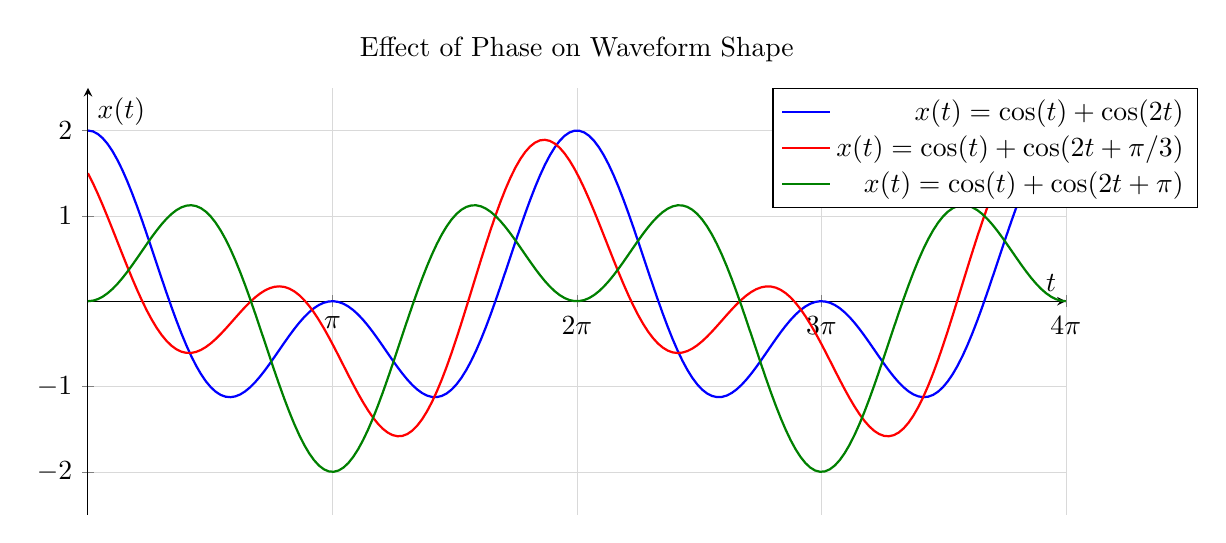
\begin{tikzpicture}
	\begin{axis}[
		width=14cm,
		height=7cm,
		title={Effect of Phase on Waveform Shape},
		xlabel={$t$},
		ylabel={$x(t)$},
		axis lines=middle,
		xmin=0, xmax=4*pi,
		ymin=-2.5, ymax=2.5,
		xtick={0, 3.14159, 6.28318, 9.42477, 12.56637},
		xticklabels={$0$,$\pi$,$2\pi$,$3\pi$,$4\pi$},
		ytick={-2,-1,1,2},
		grid=major,
		grid style={line width=.1pt, draw=gray!30},
		legend style={
			at={(0.7, 1)}, % 3% from left, 97% from bottom
			anchor=north west,   % Anchor the top-left corner of the legend
			legend cell align={right}
		},
		no marks,
		]
		% Case 1: phi = 0
		\addplot[blue, thick, domain=0:4*pi, samples=200] {cos(deg(x)) + cos(deg(2*x))};
		\addlegendentry{$x(t) = \cos(t) + \cos(2t)$};
		
		% Case 2: phi = pi/3
		\addplot[red, thick, domain=0:4*pi, samples=200] {cos(deg(x)) + cos(deg(2*x) + 60)};
		\addlegendentry{$x(t) = \cos(t) + \cos(2t + \pi/3)$};
		
		% Case 3: phi = pi
		\addplot[green!50!black, thick, domain=0:4*pi, samples=200] {cos(deg(x)) + cos(deg(2*x) + 180)};
		\addlegendentry{$x(t) = \cos(t) + \cos(2t + \pi)$};
	\end{axis}
\end{tikzpicture}

\begin{tikzpicture}
	% Define a style for the impulse plot
	\pgfplotsset{
		impulse/.style={
			ycomb, 
			blue, 
			thick, 
			mark=*, 
			mark size=2pt, 
			mark options={fill=blue}
		}
	}
	
	\begin{axis}[
		width=14cm,
		height=7cm,
		title={Magnitude Spectrum (Unaffected by Phase)},
		xlabel={$\omega$},
		ylabel={$|X(j\omega)|$},
		axis lines=middle,
		xmin=-3.5, xmax=3.5,
		ymin=0, ymax=4,
		xtick={-2,-1,1,2},
		ytick={3.14159},
		yticklabels={$\pi$},
		grid=major,
		grid style={line width=.1pt, draw=gray!30},
		]
		% Draw impulses at w = +/-1 and w = +/-2, all with height pi
		% The node near coords places the label 'π' above each impulse.
		\addplot[
		impulse,
		nodes near coords={$\pi$},
		every node near coord/.style={anchor=south, font=\small}
		] 
		coordinates {(-2,pi) (-1,pi) (1,pi) (2,pi)};
	\end{axis}
\end{tikzpicture}









	\caption{Effect of phase on signal shape: same magnitude spectrum, different time waveforms.}
	\label{fig:two_cosines_phase}
\end{figure}

Notice that:
\begin{itemize}[noitemsep]
	\item The magnitude spectrum $|X(j\omega)|$ is identical regardless of the phase $\phi$
	\item The time-domain waveform changes dramatically as $\phi$ varies
	\item This demonstrates that phase alignment determines waveform shape
\end{itemize}
\newpage
\section*{17.3 Phase Discontinuities and Unwrapping}

When working with phase in both continuous-time and discrete-time Fourier transforms, we encounter the issue of phase wrapping. The raw phase is typically computed modulo $2\pi$, resulting in discontinuities.

\begin{definition}
	\textbf{Phase Unwrapping:} The process of removing $2\pi$ discontinuities to create a continuous phase function. This applies to both CTFT ($X(j\omega)$) and DTFT ($X(e^{j\omega})$) phase representations.
\end{definition}

\begin{figure}[H]
	\centering
	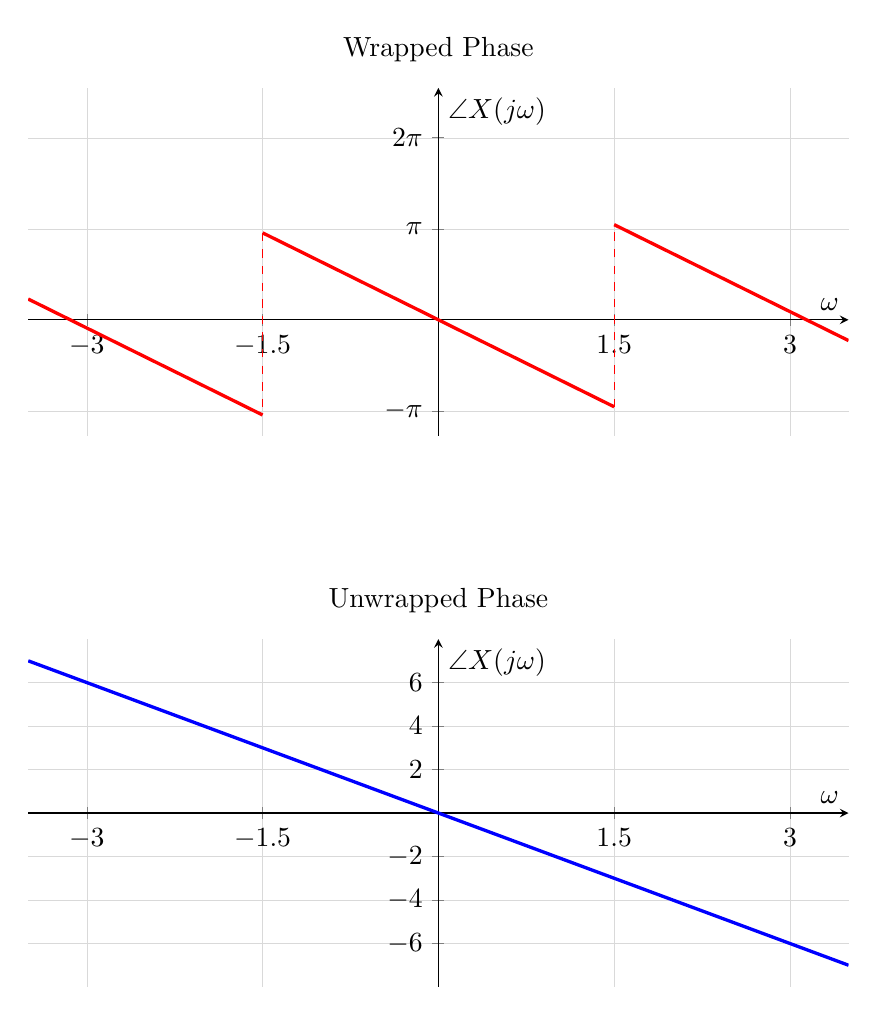
\begin{tikzpicture}
	% Define a common style
	\pgfplotsset{
		phase a/.style={
			width=12cm, height=6cm,
			axis lines=middle, xlabel={$\omega$},
			xmin=-3.5, xmax=3.5,
			xtick={-3,-1.5,1.5,3},
			grid=major, grid style={line width=.1pt, draw=gray!30},
			no marks,
		}
	}
	
	% Top plot: Wrapped Phase
	\begin{scope}[yshift=7cm]
		\begin{axis}[
			phase a,
			title={Wrapped Phase},
			ylabel={$\angle X(j\omega)$},
			ymin=-4, ymax=8,
			ytick={-3.14, 3.14, 6.28},
			yticklabels={$-\pi$, $\pi$, $2\pi$},
			]
			% Plot piecewise segments
			\addplot[red, very thick, domain=-3.5:-1.5] {-2*x - 2*pi};
			\addplot[red, very thick, domain=-1.5:1.5]  {-2*x};
			\addplot[red, very thick, domain=1.5:3.5]   {-2*x + 2*pi};
			
			% Mark discontinuities
			\draw[red, dashed] (axis cs:-1.5,3) -- (axis cs:-1.5,-3);
			\draw[red, dashed] (axis cs:1.5, -3) -- (axis cs:1.5, -3+2*pi);
		\end{axis}
	\end{scope}
	
	% Bottom plot: Unwrapped Phase
	\begin{scope}[yshift=0cm]
		\begin{axis}[
			phase a,
			title={Unwrapped Phase},
			ylabel={$\angle X(j\omega)$},
			ymin=-8, ymax=8,
			ytick={-6, -4, -2, 2, 4, 6},
			]
			\addplot[blue, very thick, domain=-3.5:3.5] {-2*x};
		\end{axis}
	\end{scope}
\end{tikzpicture}









	\caption{Wrapped vs. unwrapped phase for a complex signal.}
	\label{fig:phase_unwrapping}
\end{figure}

\paragraph{Key Points:}
\begin{itemize}[noitemsep]
	\item \textbf{Occurs in both CT and DT:} Phase wrapping and discontinuities occur in both continuous-time ($X(j\omega)$) and discrete-time ($X(e^{j\omega})$) Fourier transforms
	\item The phase plot often shows discontinuities of $2\pi$ due to "phase wrapping" (artifacts of the $\operatorname{atan2}$ function)
	\item Phase becomes ill-defined or numerically unstable at frequencies where the magnitude is zero (for CTFT: $|X(j\omega)| = 0$; for DTFT: $|X(e^{j\omega})| = 0$)
	\item Phase unwrapping is the process of removing the $2\pi$ jumps to reveal the continuous underlying phase
	\item Phase unwrapping is essential for computing derivatives (group delay: $\tau_g(\omega) = -\frac{d}{d\omega}\{\angle H(j\omega)\}$ for CTFT, or $\tau_g(\omega) = -\frac{d}{d\omega}\{\angle H(e^{j\omega})\}$ for DTFT)
	\item The unwrapped phase should be continuous and differentiable
\end{itemize}

\section*{17.4 Frequency Response}

The concepts of magnitude and phase extend naturally to LTI systems through the frequency response $H(j\omega)$.

\begin{definition}
	For an LTI system with impulse response $h(t)$, the \textbf{frequency response} is:
	\[
	H(j\omega) = \int_{-\infty}^{\infty} h(t) e^{-j\omega t} \dd t
	\]
\end{definition}

The frequency response can also be written in polar form:
\[
H(j\omega) = |H(j\omega)|e^{j\angle H(j\omega)}
\]

\begin{itemize}[noitemsep]
	\item \textbf{$|H(j\omega)|$} controls amplitude versus frequency (filtering characteristics)
	\item \textbf{$\angle H(j\omega)$} controls timing alignment (phase distortion)
\end{itemize}
\section*{Summary and Next Lecture}
	\begin{itemize}[noitemsep]
		\item The Fourier transform can be decomposed into magnitude $|X(j\omega)|$ and phase $\angle X(j\omega)$ components
		\item Magnitude tells us "what frequencies" are present in the signal
		\item Phase tells us "when frequencies align" to create the signal's shape
		\item For many signals, particularly images, phase information is more critical than magnitude
		\item Phase unwrapping is necessary for continuous phase analysis and computing group delay
		\item \textbf{Next time:} Linear phase systems, group delay, and phase distortion in LTI systems
	\end{itemize}

\end{document}
